\documentclass[12pt]{article}
\usepackage{blindtext}
\usepackage[en,bordered]{uni-style}
\usepackage{uni-math}
\usepackage{graphicx,wrapfig}


\title{\href{https://github.com/M-Sc-AUT/M.Sc-Computer-Architecture/tree/main/Embedded Systems Modeling and Design}{\textcolor{black}{Embedded Systems}}}
\prof{\href{https://scholar.google.com/citations?user=2RN0Y2YAAAAJ&hl=en}{\textcolor{black}{Prof. Sedighi}}}
\subtitle{Chapter 3 - Discrete Dynamics}
\subject{Homework 2}
\info{
    \begin{tabular}{lr}
        \href{https://github.com/M-Sc-AUT/M.Sc-Computer-Architecture/tree/main/Embedded Systems Modeling and Design}{\textcolor{black}{Reza Adinepour}} & ID: 402131055\\
    \end{tabular}
    }
    \date{\today}
    % \usepackage{xepersian}
    % \settextfont{Yas}
    \usepackage{uni-code}
    
    \begin{document}
\maketitlepage
\maketitlestart

\section{Question 2}

Consider a variant of the thermostat of example 3.5. In this variant, there is only one
temperature threshold, and to avoid chattering the thermostat simply leaves the heat
on or off for at least a fixed amount of time. In the initial state, if the temperature is
less than or equal to 20 degrees Celsius, it turns the heater on, and leaves it on for
at least 30 seconds. After that, if the temperature is greater than 20 degrees, it turns
the heater off and leaves it off for at least 2 minutes. It turns it on again only if the
temperature is less than or equal to 20 degrees.
\begin{enumerate}
	\item Design an FSM that behaves as described, assuming it reacts exactly once
	every 30 seconds.
	\begin{qsolve}[Solution]
		\begin{itemize}
			\item initial state: \textbf{colling}
			\item if $temp \le 20^{\circ} C$ $\rightarrow$ heat on $\rightarrow$ wait for 30 S
			\item if $temp > 20^{\circ} C$ $\rightarrow$ heat off $\rightarrow$ wait for 20 min on heating state
		\end{itemize}
		
	we can draw FSM as bellow:\\
	
	\centering\includegraphics*[width=0.8\linewidth]{images/img7}
	\captionof{figure}{FSM solution of part 1}
	\end{qsolve}
	
	
	
	\item How many possible states does your thermostat have? Is this the smallest
	number of states possible?
	\begin{qsolve}[Solution]
		I try to draw the smallest FSM for this problem. This FSM contain a 3 state.
	\end{qsolve}
	
	
	
	
	\item Does this model thermostat have the time-scale invariance property?
	\begin{qsolve}[Solution]
		The model does not have the hysteresis property because the timeout is a fixed amount
		of time, so varying the time scale of the input will yield distinctly different behavior.
	\end{qsolve}
\end{enumerate}


\vfil
\clearpage













\section{Question 3}
Consider the following state machine:

\centering\includegraphics*[width=0.4\linewidth]{images/img1}
\captionof{figure}{State machine of question 2}



\raggedright Determine whether the following statement is true or false, and give a supporting argument:\newline

The output will eventually be a constant 0, or it will eventually be a
constant 1. That is, for some n ∈ N, after the n-th reaction, either the
output will be 0 in every subsequent reaction, or it will be 1 in every
subsequent reaction.\newline

Note that Chapter 13 gives mechanisms for making such statements precise and for
reasoning about them.

	
\begin{qsolve}[Solution]
	Due to non-deterministic behavior of the system in state A so the destination after this state is not clear but it could be seen that eventually it is possible to reaching the state B. In state B because of deterministic behavior, it remained in this stage.
\end{qsolve}

\vfil
\clearpage












\section{Question 4}
How many reachable states does the following state machine have?\newline


\centering\includegraphics*[width=0.8\linewidth]{images/img2}
\captionof{figure}{State machine of question 4}


\begin{qsolve}[Solution]
	As we know the formula of reachable states define as follow:
	$$ |states|=np^m $$
	So we have:
	$$ |states|=3\times3^1=9 $$
	
	We have 9 reachable states in this state machine.
	
\end{qsolve}
\vfil
\clearpage

















\section{Question 5}
Consider the deterministic finite-state machine in Figure 3.14 that models a simple
traffic light.\newline


\centering\includegraphics*[width=0.6\linewidth]{images/img3}
\captionof{figure}{Deterministic finite-state machine for question 5}


\begin{enumerate}
	\item Formally write down the description of this FSM as a 5-tuple:\\
	\centering(States, Inputs, Outputs, update, initialState)
	
	\begin{qsolve}[Solution]
		\raggedright States = $\{red,\ green,\ yellow\}$ \\
		Inputs = $\{ tick \rightarrow \{present, absent \} \}$ \\
		Output = $\{\{go, stop\} \rightarrow \{present, absent\} \}$ \\
		Initial state = $\{red\}$\\
		Update = $\{\{red,green\}\rightarrow \{tick=present\}, \{green,yellow\}\rightarrow \{tick=present\}, \{yellow,red\}\rightarrow \{tick=present\} \}$
	\end{qsolve}
	
	
	\item \raggedright Give an execution trace of this FSM of length 4 assuming the input \textit{tick} is
	\textit{present} on each reaction.
	\begin{qsolve}[Solution]
		$red \ \xrightarrow{\text{tick=present/go}} \ green \xrightarrow{\text{tick=present/stop}} \ yellow \xrightarrow{\text{tick=present/stop}} \ red$
	\end{qsolve}
	
	
	
	
	\item Now consider merging the red and yellow states into a single stop state. Tran
	sitions that pointed into or out of those states are now directed into or out of
	the new stop state. Other transitions and the inputs and outputs stay the same.
	The new stop state is the new initial state. Is the resulting state machine de
	terministic? Why or why not? If it is deterministic, give a prefix of the trace
	of length 4. If it is nondeterministic, draw the computation tree up to depth 4.
	\begin{qsolve}[Solution]
		The new FSM as bellow:
		
		
		\centering\includegraphics*[width=0.6\linewidth]{images/img8}
		\captionof{figure}{New FSM of part 3}
		
		\raggedright This is the newest FSM. this is a non-deterministic FSM because two state of yellow and red are merged in new state of stop. so the stop state can do two transition with tick gard.
		\newline
		we can draw computation tree with depth 4 as bellow:
		
		\centering\includegraphics*[width=0.6\linewidth]{images/img9}
		\captionof{figure}{New FSM of part 3}
		
	\end{qsolve}
\end{enumerate}

	

	

\vfil
\clearpage


















\section{Question 6}
\raggedright This problem considers variants of the FSM in Figure 3.11, which models arrivals of pedestrians at a crosswalk. We assume that the traffic light at the crosswalk is controlled by the FSM in Figure 3.10. In all cases, assume a time triggered model, where both the pedestrian model and the traffic light model react once per second. Assume further that in each reaction, each machine sees as inputs the output produced by the other machine \textit{in the same reaction} (this form of composition, which is called synchronous composition, is studied further in Chapter 6).

\begin{enumerate}
	\item Suppose that instead of Figure 3.11, we use the following FSM to model the
	arrival of pedestrians:
	
	\centering\includegraphics*[width=0.5\linewidth]{images/img4}
	
	\raggedright Find a trace whereby a pedestrian arrives (the above machine transitions to
	waiting) but the pedestrian is never allowed to cross. That is, at no time after
	the pedestrian arrives is the traffic light in state red.
	\begin{qsolve}[Solution]
		According to the pedestrian FSM, in its initial state it has a nondeterministic condition. Hence,
		we can suppose that, at first, we are in red and none states. Although the none state can
		repeat because of nondeterministic behavior, the red state after 60 seconds transfers to the
		green state. So, suppose that in the same time the red and none states transfer to the green
		and waiting states.
	\end{qsolve}
	
	\item Suppose that instead of Figure 3.11, we use the following FSM to model the arrival of pedestrians:
	
	\centering\includegraphics*[width=0.5\linewidth]{images/img5}
	
	\raggedright Here, the initial state is nondeterministically chosen to be one of none or
	crossing. Find a trace whereby a pedestrian arrives (the above machine tran
	sitions from none to waiting) but the pedestrian is never allowed to cross. That
	is, at no time after the pedestrian arrives is the traffic light in state red.
	\begin{qsolve}[Solution]
		Suppose that we are in state none and red for pedestrian and traffic light respectively. At first,
		it could transition to waiting and red states because of nondeterministically behavior. After
		that, the red state transfer to the green state.	
	\end{qsolve}
\end{enumerate}
\vfil
\clearpage




















\section{Question 7}
Consider the state machine in Figure 7 State whether each of the following is
a behavior for this machine. In each of the following, the ellipsis “...” means that
the last symbol is repeated forever. Also, for readability, \textit{absent} is denoted by the
shorthand $a$ and \textit{present} by the shorthand $p$.


\begin{enumerate}
	\item $x=(p,p,p,p,p,...),\ \ y=(0,1,1,0,0,...)$
	\begin{qsolve}[Solution]
		This is not behavior for this machine	
	\end{qsolve}
	
	\item $x=(p,p,p,p,p,...),\ \ y=(0,1,1,0,a,...)$
	\begin{qsolve}[Solution]
		This is behavior for this machine	
	\end{qsolve}
	
	\item $x=(a,p,a,p,a,...),\ \ y=(a,1,a,0,a,...)$
	\begin{qsolve}[Solution]
		This is not behavior for this machine	
	\end{qsolve}
	
	\item $x=(p,p,p,p,p,...),\ \ y=(0,0,a,a,a,...)$
	\begin{qsolve}[Solution]
		This is behavior for this machine	
	\end{qsolve}
	
	\item $x=(p,p,p,p,p,...),\ \ y=(0,a,0,a,a,...)$
	\begin{qsolve}[Solution]
		This is behavior for this machine	
	\end{qsolve}
\end{enumerate}

\centering\includegraphics*[width=0.6\linewidth]{images/img6}
\captionof{figure}{State machine for question 7}

%\begin{figure}[h]
%	\centering
%	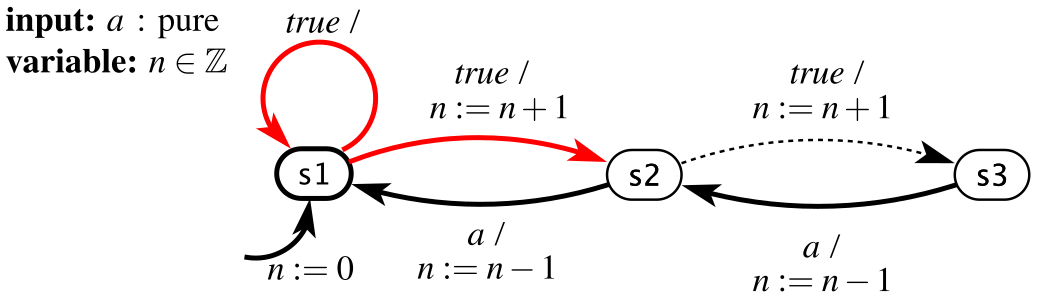
\includegraphics[width=0.7\textwidth]{images/img2}
%	\caption{A PI controller for the helicopter}
%	\label{fig:A PI controller for the helicopter}
%\end{figure}


\vfil
\clearpage























\section{Question 8}
(NOTE: This exercise is rather advanced.) This exercise studies properties of dis
crete signals as formally defined in the sidebar on page 45. Specifically, we will
show that discreteness is not a compositional property. That is, when combining
two discrete behaviors in a single system, the resulting combination is not neces
sarily discrete.


\begin{enumerate}
	\item Consider a pure signal $x:\mathbb{R} \rightarrow \{present, absent\}$ given by:\\
	$$
	x(t)=
	\begin{cases}
		present \ \ \  \texttt{if $t$ is a non-negative integer} \\
		absent \ \ \    \texttt{otherwise}\\
	\end{cases}
	$$
	
	for all $t \in \mathbb{R}$. Show that this signal is discrete.
	
	
	
	
	\item Consider a pure signal $y:\mathbb{R} \rightarrow \{present, absent\}$ given by:\\
	$$
	y(t)=
	\begin{cases}
		present \ \ \  \texttt{if $t=1-1/n$ for any positive integer $n$} \\
		absent \ \ \    \texttt{otherwise}\\
	\end{cases}
	$$
	
	for all $t \in \mathbb{R}$. Show that this signal is discrete.
	
	
	
	
	\item Consider a signal $\omega$ that is the merge of $x$ and $y$ in the previous two parts.
	That is, $w(t)=present$ if either $x(t) = present$ or $y(t) = present$, and is
	\textit{absent} otherwise. Show that $\omega$ is not discrete.
	
	
	
	\item Consider the example shown in Figure 3.1. Assume that each of the two
	signals \textit{arrival} and \textit{departure} is discrete. Show that this does not imply that
	the output \textit{count} is a discrete signal.
	
	
	
	
\end{enumerate}

%\begin{figure}[h]
%	\centering
%	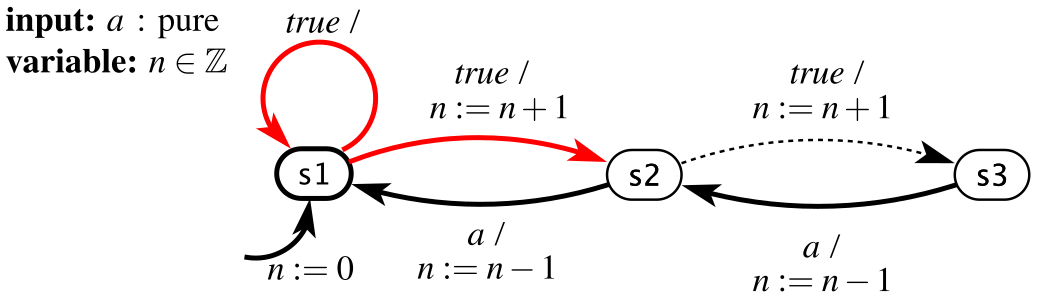
\includegraphics[width=0.7\textwidth]{images/img2}
%	\caption{A PI controller for the helicopter}
%	\label{fig:A PI controller for the helicopter}
%\end{figure}



\begin{qsolve}[Solution]
	I so sorry. I don't have any idea for this question.
\end{qsolve}
\vfil
\clearpage




\vspace*{\fill}
\begin{center}
	\makeendpage

\end{center}
\vfill % equivalent to \vspace{\fill}
\clearpage




\end{document}